\begin{table*}[b]
	\centering
	\renewcommand{\arraystretch}{1.3}
	\begin{tabularx}{\textwidth}{|Y|Y|Y|Y|}
		\hline
		
		\textbf{Scenario} 1 & \textbf{Scenario 2} & \textbf{Scenario 3} & \textbf{Scenario 4} \\
		
		\hline
		
		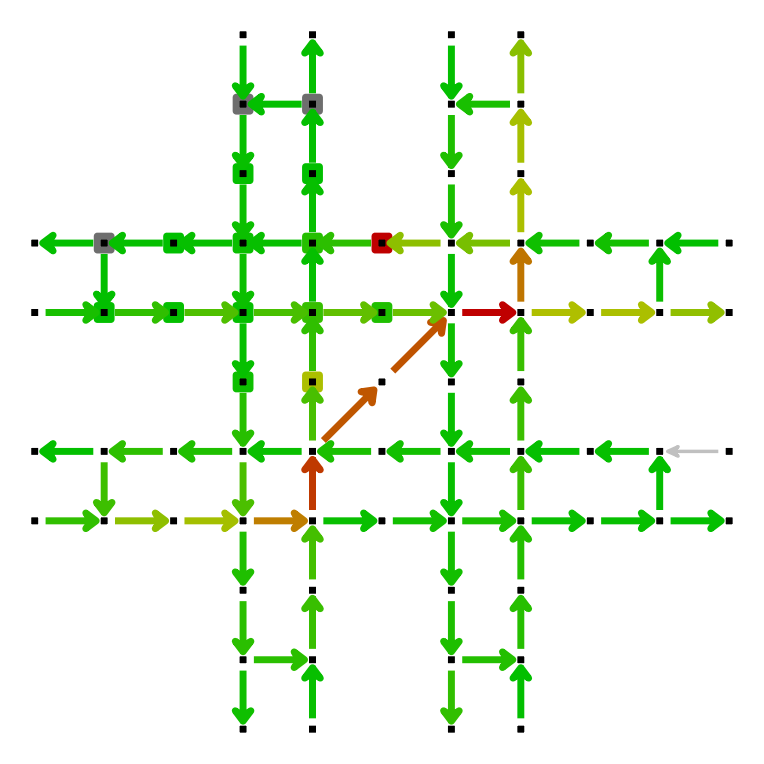
\includegraphics[width=0.23\textwidth]{../gfx/data/E1_003.png} &
		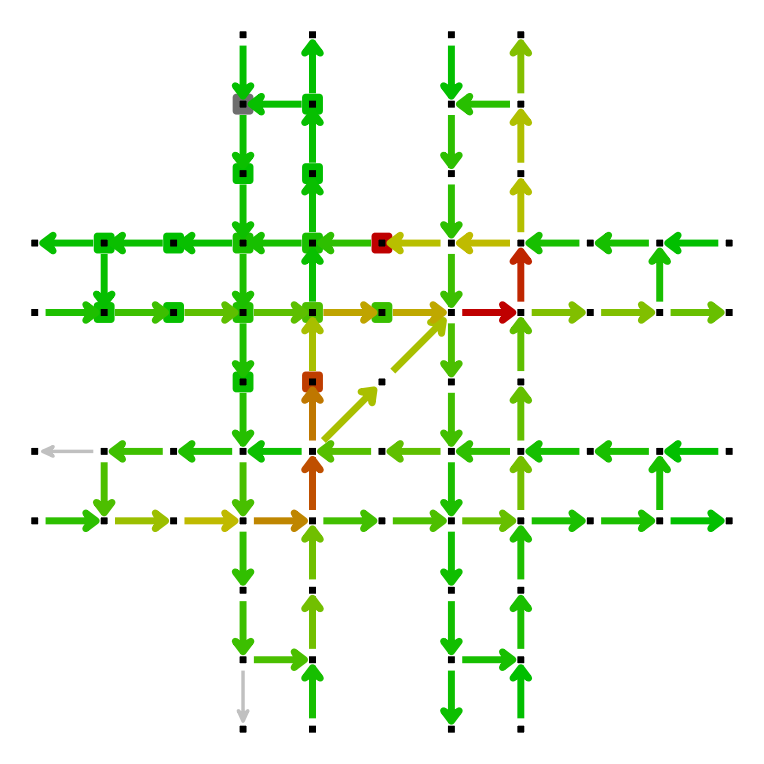
\includegraphics[width=0.23\textwidth]{../gfx/data/E2_003.png} &
		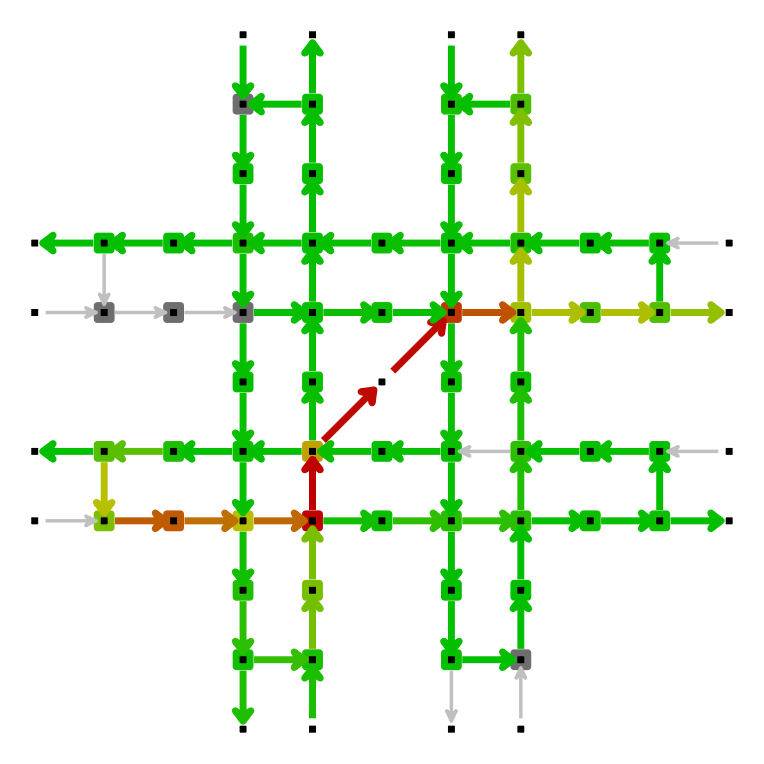
\includegraphics[width=0.23\textwidth]{../gfx/data/E3_003.png} &
		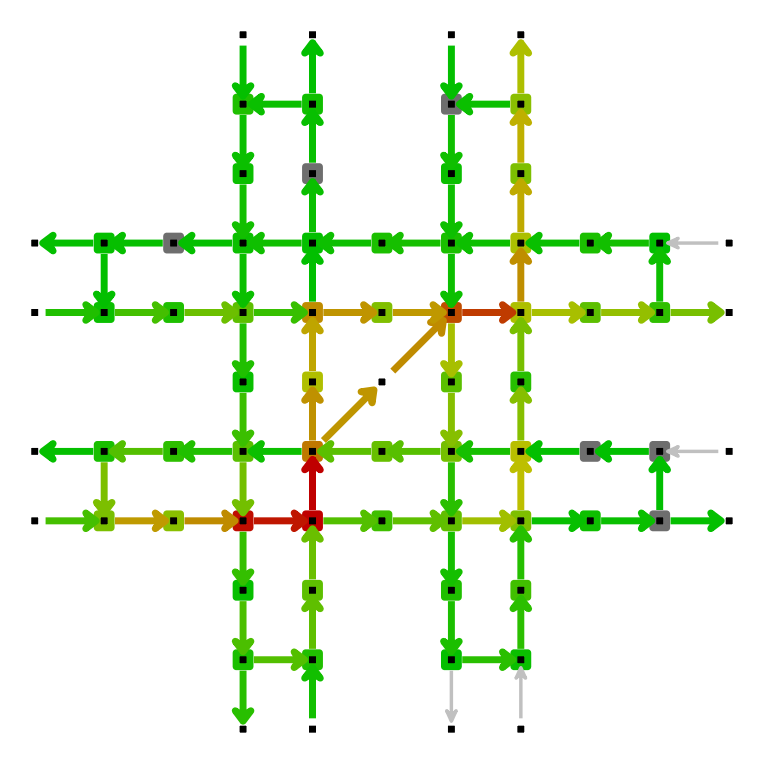
\includegraphics[width=0.23\textwidth]{../gfx/data/E4_003.png} \\
		
		\hline
		
		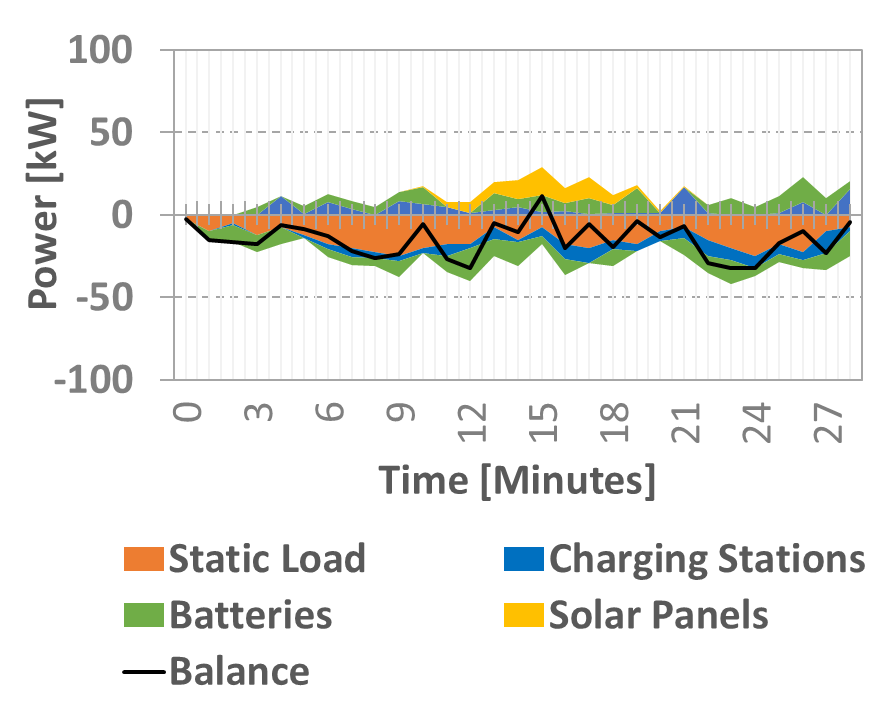
\includegraphics[width=0.23\textwidth]{../gfx/data/E1_001.png} &
		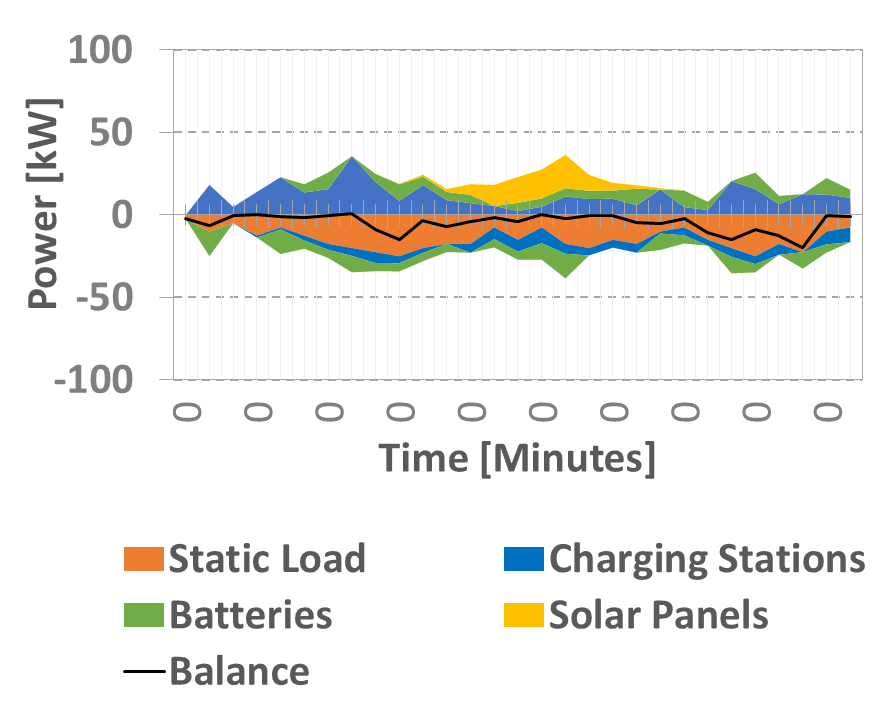
\includegraphics[width=0.23\textwidth]{../gfx/data/E2_001.png} &
		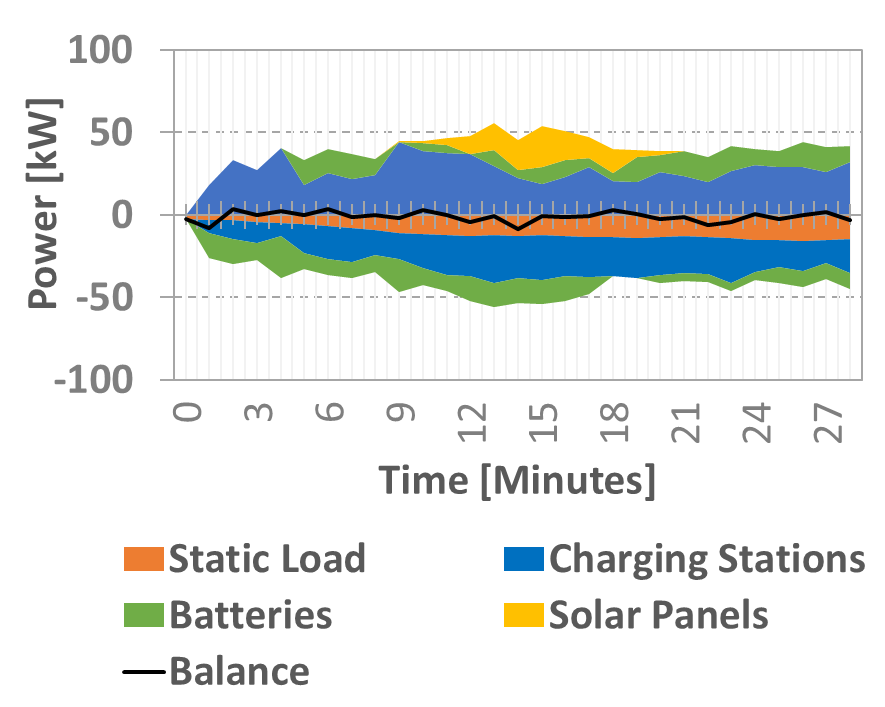
\includegraphics[width=0.23\textwidth]{../gfx/data/E3_001.png} &
		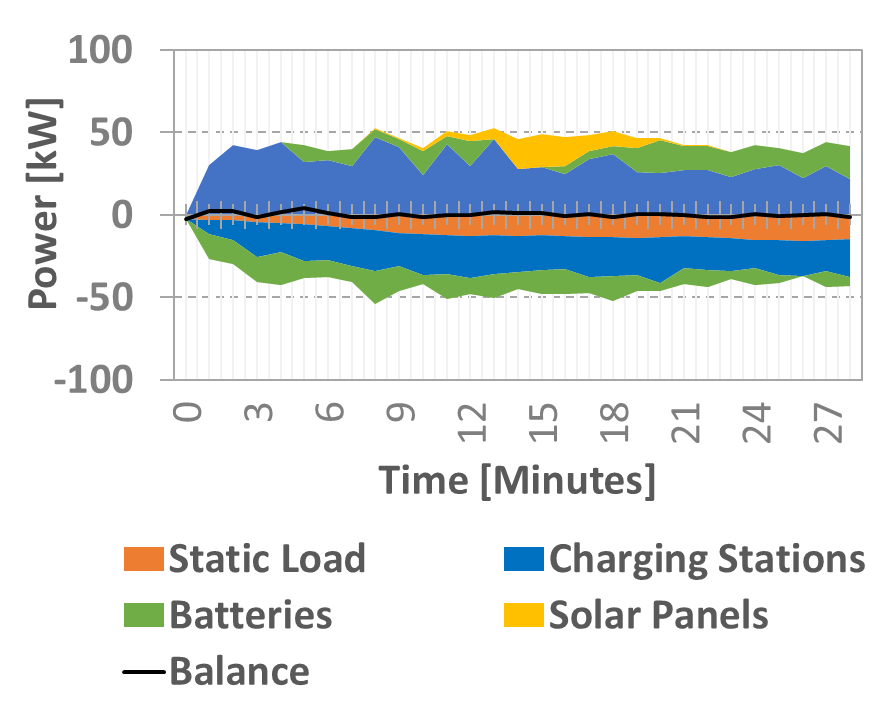
\includegraphics[width=0.23\textwidth]{../gfx/data/E4_001.png} \\
		
		\hline
		
		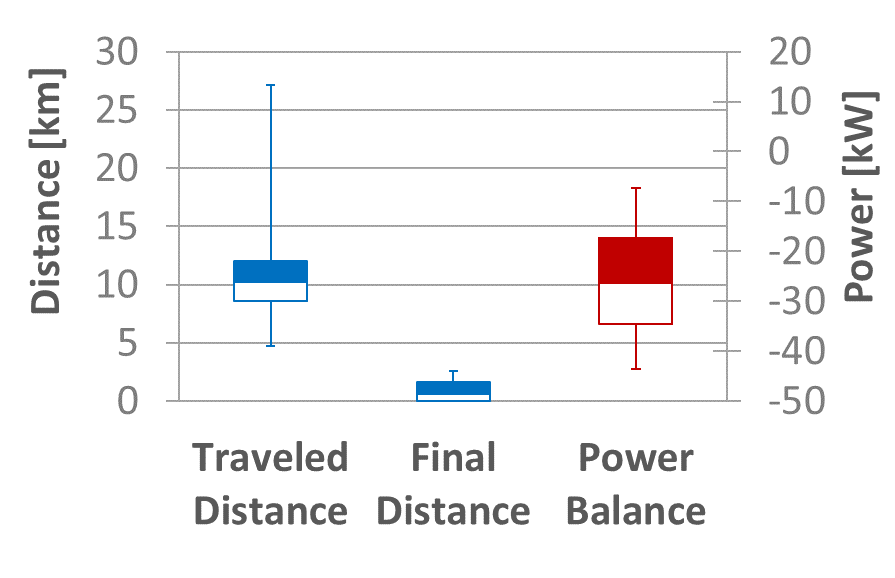
\includegraphics[width=0.23\textwidth]{../gfx/data/E1_002.png} &
		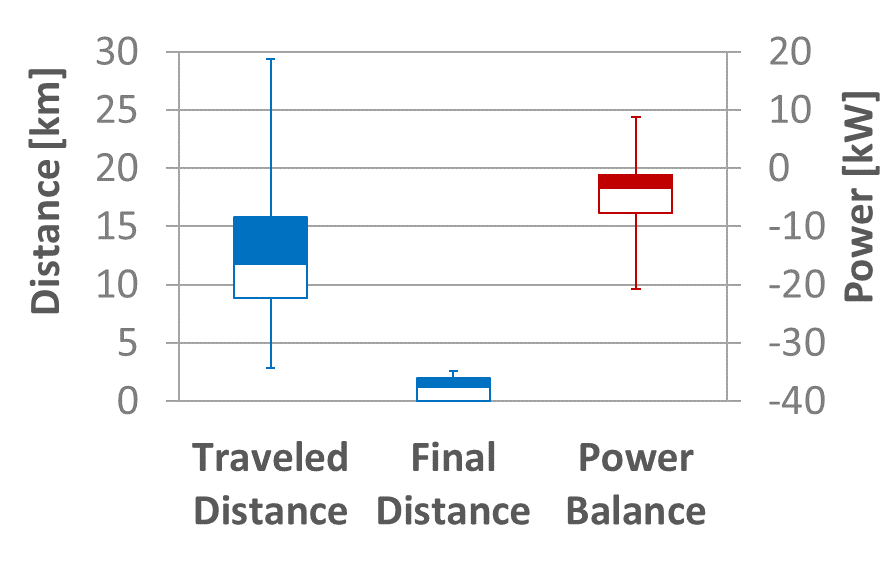
\includegraphics[width=0.23\textwidth]{../gfx/data/E2_002.png} &
		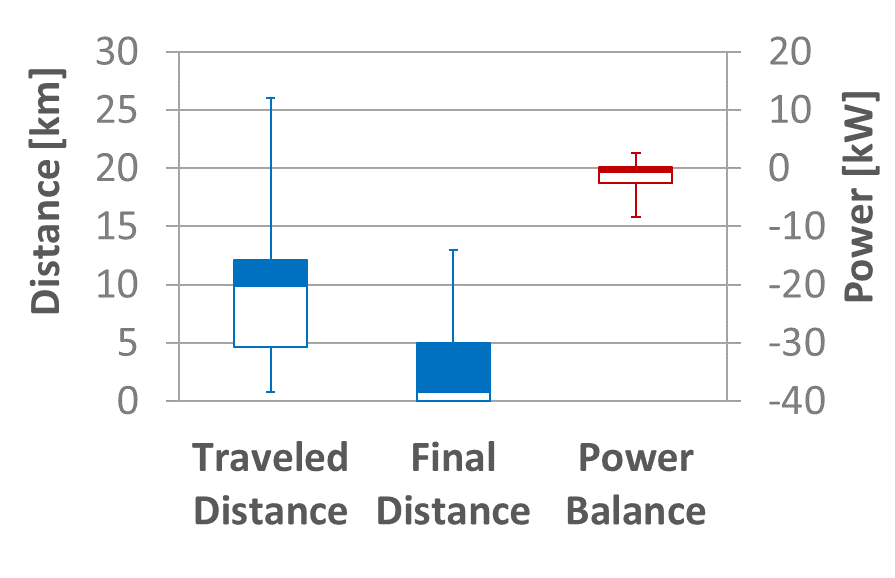
\includegraphics[width=0.23\textwidth]{../gfx/data/E3_002.png} &
		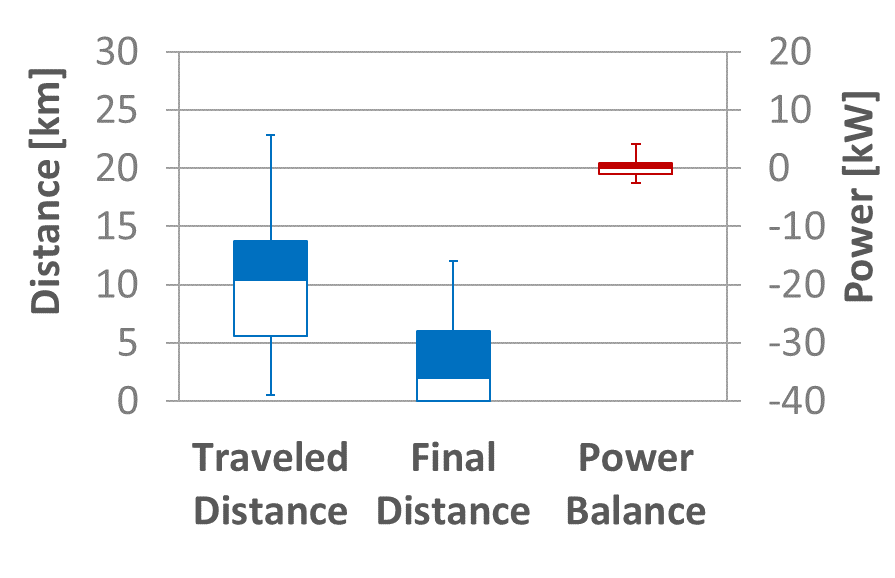
\includegraphics[width=0.23\textwidth]{../gfx/data/E4_002.png} \\
		
		\hline
		
		\begin{tabulary}{4cm}{L|L}
			\textit{Computation time} & 229s \\
			\textit{Memory usage} & 6.03GB \\
			\textit{Lines of code} & 350 \\
		\end{tabulary}
		&
		\begin{tabulary}{4cm}{L|L}
			\textit{Computation time} & 250s \\
			\textit{Memory usage} & 5.27GB \\
			\textit{Lines of code} & 350 \\
		\end{tabulary}
		&
		\begin{tabulary}{4cm}{L|L}
			\textit{Computation time} & 218s \\
			\textit{Memory usage} & 6.41GB \\
			\textit{Lines of code} & 350 \\
		\end{tabulary}
		&
		\begin{tabulary}{4cm}{L|L}
			\textit{Computation time} & 227s \\
			\textit{Memory usage} & 6.75GB \\
			\textit{Lines of code} & 350 \\
		\end{tabulary}
		\\
		
		\hline
	\end{tabularx}
	\caption{Traffic flow graph, power chart, statistics, computation time, memory usage, and lines of code for each scenario.}
	\label{figure:examples}
\end{table*}

\section{Demonstration}
\label{section:evaluation}

To demonstrate the presented approach, we provide four examples with specific scenario configurations. Generally, all examples are simulated with a time resolution of 60 seconds per simulation step and 30 simulation steps in total, aggregating to a total duration of 30 minutes. The examples evaluate the effects of varying the weights $w\_TS$ and $w\_PS$ between the transportation system cost and the power system cost as well as the state of expansion of the power system.

To model the stage of expansion of the power system, between Scenarios 1-2 and Scenarios 3-4 the parameters of power system $PS$ are varied in terms of the number of charging stations $CS\_Number$ as well as in terms of solar panel capacities $Power\_Scale$ and power battery capacities $SOC\_Max$. Moreover, all scenarios include ten static load components, five solar panel components and five power battery components represented through their configurations $SL_{A}$, $SP_{A}$ and $PB_{A}$ or their respective stages of expansion $SL_{B}$, $SP_{B}$ and $PB_{B}$. From Scenarios 1-2 to Scenarios 3-4, solar panel capacities are increased twofold, while battery capacities are increased fourfold. Furthermore, in Scenarios 1-2 16 charging stations are employed, while Scenarios 3-4 utilize 56 charging stations. In all scenarios charging stations with reference configuration $CS_{A}$ are used. In terms of the electricity infrastructure, for low-voltage nets with configuration $LV_{A}$ and one medium-voltage net with configuration $MV_{A}$ are employed in all scenarios. 

In terms of the transportation system $TS$, the examples feature a total number of 440 cars $C$. The cars are distributed equally among the reference configurations $C_{A}$, $C_{B}$ and $C_{C}$. There reference configurations mainly differ in the initial state of charge $SOC$ with 33\%, 66\% and 100\% of the maximum state of charge $SOC\_Max$ respectively. In terms of positioning on the traffic network $TN$, the origin positions $Origin$ of cars are drawn randomly from all edges $E$ present within the traffic network. Instead, the destination positions $Destination$ are drawn randomly from the set of the eight most outward edges of the traffic network. Finally, for origins we prefer the lower left sector of $TN$, while for destinations we prefer the upper right sector of $TN$.

The results of control optimization are shown in Tab.~\ref{figure:examples}. For each scenario, a traffic flow graph and power chart is provided as well as general statistics and performance characteristics.

\subsection*{Scenario 1: Prefer trans.\ system, low stage of expansion}

Scenario~1 describes an example with a low number and low capacities of smart and renewable energy devices. That is, solar panel and power battery capacity available within the power system is low, while static profiles within the power system have high impact in terms of intermittent power loads. Furthermore, only a low number of charging stations is available within the transportation system. In terms of costs, in benefit of achieving the objectives of the transportation system, more weight is assigned to the costs incurred by the transportation instead of the power system. Behavior estimation results show high frequency of routes using shortest paths to destinations. Power balance is prone to high and sudden fluctuations in load. Little equalization of net balances is made by cars charging or discharging at charging stations.

\subsection*{Scenario 2: Prefer power system, low stage of expansion}

Different to Scenario~1, in benefit of achieving the objectives of the power system, more weight is assigned to the costs incurred by power system instead of the transportation system. Behavior estimation results show higher frequency of edges around and on charging stations. Furthermore, compared to Scenario~1, cars utilize shortest path routes less frequently, which results in marginally higher distance traveled by cars. Also in contrast to Scenario~1, negative power balances are equalized to a higher level, traceable to cars discharging at charging stations and therefore supporting equalized net balance.

\subsection*{Scenario 3: Prefer trans.\ system, high stage of expansion}

In Scenario~3 additional solar panel and power battery capacity as well as a higher number of charging stations are employed. As the power grid and it's electric devices get smarter, the profiles of static loads are more evened out, as less intermittent power load peaks occur. In benefit of achieving the objectives of the transportation system, more weight is assigned to the costs incurred by transportation system instead of the power system. Similar to Scenario~1, behavior estimation results show high frequency of routes using shortest paths to destinations. Overall distance traveled by cars is decreased, while final distance to destination is increased. Compared to Scenario~2, a higher level of equalization of power balance can be observed, due to higher energy device count and capacities.

\subsection*{Scenario 4: Prefer power system, high stage of expansion}

In Scenario 4 more weight is assigned to the costs incurred by power system instead of the transportation system. Similar to results observed in Scenario~2, behavior estimation results show that cars utilize shortest path routes less frequently compared to Scenarios~1 and~3, which results in marginally higher distance traveled and final distance to destination. However, compared to Scenario~2, frequency is distributed more evenly across the traffic network, resulting in higher frequency of edges around and on charging stations compared to Scenario~3. Furthermore, due to higher utilization of charging stations, in contrast to Scenario~3, net balances are equalized to a higher degree.